\PassOptionsToPackage{unicode=true}{hyperref} % options for packages loaded elsewhere
\PassOptionsToPackage{hyphens}{url}
%
\documentclass[
]{article}
\usepackage{lmodern}
\usepackage{amssymb,amsmath}
\usepackage{ifxetex,ifluatex}
\ifnum 0\ifxetex 1\fi\ifluatex 1\fi=0 % if pdftex
  \usepackage[T1]{fontenc}
  \usepackage[utf8]{inputenc}
  \usepackage{textcomp} % provides euro and other symbols
\else % if luatex or xelatex
  \usepackage{unicode-math}
  \defaultfontfeatures{Scale=MatchLowercase}
  \defaultfontfeatures[\rmfamily]{Ligatures=TeX,Scale=1}
\fi
% use upquote if available, for straight quotes in verbatim environments
\IfFileExists{upquote.sty}{\usepackage{upquote}}{}
\IfFileExists{microtype.sty}{% use microtype if available
  \usepackage[]{microtype}
  \UseMicrotypeSet[protrusion]{basicmath} % disable protrusion for tt fonts
}{}
\makeatletter
\@ifundefined{KOMAClassName}{% if non-KOMA class
  \IfFileExists{parskip.sty}{%
    \usepackage{parskip}
  }{% else
    \setlength{\parindent}{0pt}
    \setlength{\parskip}{6pt plus 2pt minus 1pt}}
}{% if KOMA class
  \KOMAoptions{parskip=half}}
\makeatother
\usepackage{xcolor}
\IfFileExists{xurl.sty}{\usepackage{xurl}}{} % add URL line breaks if available
\IfFileExists{bookmark.sty}{\usepackage{bookmark}}{\usepackage{hyperref}}
\hypersetup{
  pdftitle={Practice 2 (partially completed)},
  pdfborder={0 0 0},
  breaklinks=true}
\urlstyle{same}  % don't use monospace font for urls
\usepackage[margin=1in]{geometry}
\usepackage{color}
\usepackage{fancyvrb}
\newcommand{\VerbBar}{|}
\newcommand{\VERB}{\Verb[commandchars=\\\{\}]}
\DefineVerbatimEnvironment{Highlighting}{Verbatim}{commandchars=\\\{\}}
% Add ',fontsize=\small' for more characters per line
\usepackage{framed}
\definecolor{shadecolor}{RGB}{248,248,248}
\newenvironment{Shaded}{\begin{snugshade}}{\end{snugshade}}
\newcommand{\AlertTok}[1]{\textcolor[rgb]{0.94,0.16,0.16}{#1}}
\newcommand{\AnnotationTok}[1]{\textcolor[rgb]{0.56,0.35,0.01}{\textbf{\textit{#1}}}}
\newcommand{\AttributeTok}[1]{\textcolor[rgb]{0.77,0.63,0.00}{#1}}
\newcommand{\BaseNTok}[1]{\textcolor[rgb]{0.00,0.00,0.81}{#1}}
\newcommand{\BuiltInTok}[1]{#1}
\newcommand{\CharTok}[1]{\textcolor[rgb]{0.31,0.60,0.02}{#1}}
\newcommand{\CommentTok}[1]{\textcolor[rgb]{0.56,0.35,0.01}{\textit{#1}}}
\newcommand{\CommentVarTok}[1]{\textcolor[rgb]{0.56,0.35,0.01}{\textbf{\textit{#1}}}}
\newcommand{\ConstantTok}[1]{\textcolor[rgb]{0.00,0.00,0.00}{#1}}
\newcommand{\ControlFlowTok}[1]{\textcolor[rgb]{0.13,0.29,0.53}{\textbf{#1}}}
\newcommand{\DataTypeTok}[1]{\textcolor[rgb]{0.13,0.29,0.53}{#1}}
\newcommand{\DecValTok}[1]{\textcolor[rgb]{0.00,0.00,0.81}{#1}}
\newcommand{\DocumentationTok}[1]{\textcolor[rgb]{0.56,0.35,0.01}{\textbf{\textit{#1}}}}
\newcommand{\ErrorTok}[1]{\textcolor[rgb]{0.64,0.00,0.00}{\textbf{#1}}}
\newcommand{\ExtensionTok}[1]{#1}
\newcommand{\FloatTok}[1]{\textcolor[rgb]{0.00,0.00,0.81}{#1}}
\newcommand{\FunctionTok}[1]{\textcolor[rgb]{0.00,0.00,0.00}{#1}}
\newcommand{\ImportTok}[1]{#1}
\newcommand{\InformationTok}[1]{\textcolor[rgb]{0.56,0.35,0.01}{\textbf{\textit{#1}}}}
\newcommand{\KeywordTok}[1]{\textcolor[rgb]{0.13,0.29,0.53}{\textbf{#1}}}
\newcommand{\NormalTok}[1]{#1}
\newcommand{\OperatorTok}[1]{\textcolor[rgb]{0.81,0.36,0.00}{\textbf{#1}}}
\newcommand{\OtherTok}[1]{\textcolor[rgb]{0.56,0.35,0.01}{#1}}
\newcommand{\PreprocessorTok}[1]{\textcolor[rgb]{0.56,0.35,0.01}{\textit{#1}}}
\newcommand{\RegionMarkerTok}[1]{#1}
\newcommand{\SpecialCharTok}[1]{\textcolor[rgb]{0.00,0.00,0.00}{#1}}
\newcommand{\SpecialStringTok}[1]{\textcolor[rgb]{0.31,0.60,0.02}{#1}}
\newcommand{\StringTok}[1]{\textcolor[rgb]{0.31,0.60,0.02}{#1}}
\newcommand{\VariableTok}[1]{\textcolor[rgb]{0.00,0.00,0.00}{#1}}
\newcommand{\VerbatimStringTok}[1]{\textcolor[rgb]{0.31,0.60,0.02}{#1}}
\newcommand{\WarningTok}[1]{\textcolor[rgb]{0.56,0.35,0.01}{\textbf{\textit{#1}}}}
\usepackage{graphicx,grffile}
\makeatletter
\def\maxwidth{\ifdim\Gin@nat@width>\linewidth\linewidth\else\Gin@nat@width\fi}
\def\maxheight{\ifdim\Gin@nat@height>\textheight\textheight\else\Gin@nat@height\fi}
\makeatother
% Scale images if necessary, so that they will not overflow the page
% margins by default, and it is still possible to overwrite the defaults
% using explicit options in \includegraphics[width, height, ...]{}
\setkeys{Gin}{width=\maxwidth,height=\maxheight,keepaspectratio}
\setlength{\emergencystretch}{3em}  % prevent overfull lines
\providecommand{\tightlist}{%
  \setlength{\itemsep}{0pt}\setlength{\parskip}{0pt}}
\setcounter{secnumdepth}{-2}
% Redefines (sub)paragraphs to behave more like sections
\ifx\paragraph\undefined\else
  \let\oldparagraph\paragraph
  \renewcommand{\paragraph}[1]{\oldparagraph{#1}\mbox{}}
\fi
\ifx\subparagraph\undefined\else
  \let\oldsubparagraph\subparagraph
  \renewcommand{\subparagraph}[1]{\oldsubparagraph{#1}\mbox{}}
\fi

% set default figure placement to htbp
\makeatletter
\def\fps@figure{htbp}
\makeatother


\title{Practice 2 (partially completed)}
\author{}
\date{\vspace{-2.5em}}

\begin{document}
\maketitle

\hypertarget{problem-1}{%
\section{Problem 1}\label{problem-1}}

\hypertarget{ex-1.1-compute-the-mean-tooth-length-for-all-six-combinations-of-supplement-types-and-levels.-also-provide-the-standard-error-of-the-mean-for-each-situation.}{%
\subsection{Ex 1.1 Compute the mean tooth length for all six
combinations of supplement types and levels. Also provide the standard
error of the mean for each
situation.}\label{ex-1.1-compute-the-mean-tooth-length-for-all-six-combinations-of-supplement-types-and-levels.-also-provide-the-standard-error-of-the-mean-for-each-situation.}}

\begin{Shaded}
\begin{Highlighting}[]
\KeywordTok{head}\NormalTok{(ToothGrowth)}
\end{Highlighting}
\end{Shaded}

\begin{verbatim}
##    len supp dose
## 1  4.2   VC  0.5
## 2 11.5   VC  0.5
## 3  7.3   VC  0.5
## 4  5.8   VC  0.5
## 5  6.4   VC  0.5
## 6 10.0   VC  0.5
\end{verbatim}

\begin{Shaded}
\begin{Highlighting}[]
\NormalTok{ToothGrowth}\OperatorTok{$}\NormalTok{dose <-}\StringTok{ }\KeywordTok{as.factor}\NormalTok{(ToothGrowth}\OperatorTok{$}\NormalTok{dose)}

\NormalTok{dose_}\FloatTok{0.5}\NormalTok{ <-}\StringTok{ }\NormalTok{ToothGrowth}\OperatorTok{$}\NormalTok{dose }\OperatorTok{==}\StringTok{ }\FloatTok{0.5}
\NormalTok{dose_}\FloatTok{1.0}\NormalTok{ <-}\StringTok{ }\NormalTok{ToothGrowth}\OperatorTok{$}\NormalTok{dose }\OperatorTok{==}\StringTok{ }\FloatTok{1.0}
\NormalTok{dose_}\FloatTok{2.0}\NormalTok{ <-}\StringTok{ }\NormalTok{ToothGrowth}\OperatorTok{$}\NormalTok{dose }\OperatorTok{==}\StringTok{ }\FloatTok{2.0}

\NormalTok{supp_vc <-}\StringTok{ }\NormalTok{ToothGrowth}\OperatorTok{$}\NormalTok{supp }\OperatorTok{==}\StringTok{ "VC"}
\NormalTok{supp_oj <-}\StringTok{ }\NormalTok{ToothGrowth}\OperatorTok{$}\NormalTok{supp }\OperatorTok{==}\StringTok{ "OJ"}

\CommentTok{# supp VC}
\NormalTok{supp_}\FloatTok{0.5}\NormalTok{vc <-}\StringTok{ }\NormalTok{supp_vc }\OperatorTok{&}\StringTok{ }\NormalTok{dose_}\FloatTok{0.5}
\NormalTok{supp_}\FloatTok{1.0}\NormalTok{vc <-}\StringTok{ }\NormalTok{supp_vc }\OperatorTok{&}\StringTok{ }\NormalTok{dose_}\FloatTok{1.0}
\NormalTok{supp_}\FloatTok{2.0}\NormalTok{vc <-}\StringTok{ }\NormalTok{supp_vc }\OperatorTok{&}\StringTok{ }\NormalTok{dose_}\FloatTok{2.0}
\CommentTok{# supp OJ}
\NormalTok{supp_}\FloatTok{0.5}\NormalTok{oj <-}\StringTok{ }\NormalTok{supp_oj }\OperatorTok{&}\StringTok{ }\NormalTok{dose_}\FloatTok{0.5}
\NormalTok{supp_}\FloatTok{1.0}\NormalTok{oj <-}\StringTok{ }\NormalTok{supp_oj }\OperatorTok{&}\StringTok{ }\NormalTok{dose_}\FloatTok{1.0}
\NormalTok{supp_}\FloatTok{2.0}\NormalTok{oj <-}\StringTok{ }\NormalTok{supp_oj }\OperatorTok{&}\StringTok{ }\NormalTok{dose_}\FloatTok{2.0}

\CommentTok{# Split the dataframes}
\NormalTok{supp_}\FloatTok{0.5}\NormalTok{vc_df <-}\StringTok{ }\NormalTok{ToothGrowth[supp_}\FloatTok{0.5}\NormalTok{vc,]}
\NormalTok{supp_}\FloatTok{1.0}\NormalTok{vc_df <-}\StringTok{ }\NormalTok{ToothGrowth[supp_}\FloatTok{1.0}\NormalTok{vc,]}
\NormalTok{supp_}\FloatTok{2.0}\NormalTok{vc_df <-}\StringTok{ }\NormalTok{ToothGrowth[supp_}\FloatTok{2.0}\NormalTok{vc,]}

\NormalTok{supp_}\FloatTok{0.5}\NormalTok{oj_df <-}\StringTok{ }\NormalTok{ToothGrowth[supp_}\FloatTok{0.5}\NormalTok{oj,]}
\NormalTok{supp_}\FloatTok{1.0}\NormalTok{oj_df <-}\StringTok{ }\NormalTok{ToothGrowth[supp_}\FloatTok{1.0}\NormalTok{oj,]}
\NormalTok{supp_}\FloatTok{2.0}\NormalTok{oj_df <-}\StringTok{ }\NormalTok{ToothGrowth[supp_}\FloatTok{2.0}\NormalTok{oj,]}

\CommentTok{# list of df}
\NormalTok{list.df <-}\StringTok{ }\KeywordTok{list}\NormalTok{(supp_}\FloatTok{0.5}\NormalTok{vc_df, supp_}\FloatTok{1.0}\NormalTok{vc_df, supp_}\FloatTok{2.0}\NormalTok{vc_df, }
\NormalTok{             supp_}\FloatTok{0.5}\NormalTok{oj_df, supp_}\FloatTok{1.0}\NormalTok{oj_df, supp_}\FloatTok{2.0}\NormalTok{oj_df)}
\CommentTok{# get mean}
\NormalTok{mean.len <-}\StringTok{ }\KeywordTok{sapply}\NormalTok{(list.df, }\ControlFlowTok{function}\NormalTok{(x) }\KeywordTok{mean}\NormalTok{(x}\OperatorTok{$}\NormalTok{len))}
\CommentTok{# get se mean              # standard error of the mean = standard deviation of len / sqrt (n.data)}
\NormalTok{sd.len <-}\StringTok{ }\KeywordTok{sapply}\NormalTok{(list.df, }\ControlFlowTok{function}\NormalTok{(x) }\KeywordTok{sd}\NormalTok{(x}\OperatorTok{$}\NormalTok{len) }\OperatorTok{/}\StringTok{ }\KeywordTok{sqrt}\NormalTok{(}\KeywordTok{nrow}\NormalTok{(x)))}

\KeywordTok{data.frame}\NormalTok{(}\DataTypeTok{combinations =} \KeywordTok{c}\NormalTok{(}\StringTok{"0.5 VC"}\NormalTok{, }\StringTok{"1 VC"}\NormalTok{, }\StringTok{"2 VC"}\NormalTok{, }
                            \StringTok{"0.5 OJ"}\NormalTok{, }\StringTok{"1 OJ"}\NormalTok{, }\StringTok{"2 OJ"}\NormalTok{), }
           \DataTypeTok{mean_len =}\NormalTok{ mean.len, }
           \DataTypeTok{mean_se =}\NormalTok{ sd.len)}
\end{Highlighting}
\end{Shaded}

\begin{verbatim}
##   combinations mean_len   mean_se
## 1       0.5 VC     7.98 0.8685620
## 2         1 VC    16.77 0.7954104
## 3         2 VC    26.14 1.5171757
## 4       0.5 OJ    13.23 1.4102837
## 5         1 OJ    22.70 1.2367520
## 6         2 OJ    26.06 0.8396031
\end{verbatim}

\begin{Shaded}
\begin{Highlighting}[]
\CommentTok{# or from Gherardo solution}
\NormalTok{combinations <-}\StringTok{ }\KeywordTok{expand.grid}\NormalTok{(}\DataTypeTok{supp =} \KeywordTok{levels}\NormalTok{(ToothGrowth}\OperatorTok{$}\NormalTok{supp), }\DataTypeTok{dose =} \KeywordTok{levels}\NormalTok{(ToothGrowth}\OperatorTok{$}\NormalTok{dose))}

\NormalTok{temp <-}\StringTok{ }\KeywordTok{apply}\NormalTok{(combinations, }\DataTypeTok{MARGIN =} \DecValTok{1}\NormalTok{, }\ControlFlowTok{function}\NormalTok{(x)\{ }
\NormalTok{  ix <-}\StringTok{ }\NormalTok{ToothGrowth}\OperatorTok{$}\NormalTok{supp }\OperatorTok{==}\StringTok{ }\NormalTok{x[}\DecValTok{1}\NormalTok{] }\OperatorTok{&}\StringTok{ }\NormalTok{ToothGrowth}\OperatorTok{$}\NormalTok{dose }\OperatorTok{==}\StringTok{ }\NormalTok{x[}\DecValTok{2}\NormalTok{]}
\KeywordTok{return}\NormalTok{( }\KeywordTok{c}\NormalTok{(}\DataTypeTok{mean =} \KeywordTok{mean}\NormalTok{(ToothGrowth[ix, }\DecValTok{1}\NormalTok{]), }\DataTypeTok{se =} \KeywordTok{sd}\NormalTok{(ToothGrowth[ix, }\DecValTok{1}\NormalTok{]) }\OperatorTok{/}\StringTok{ }\KeywordTok{sqrt}\NormalTok{(}\KeywordTok{sum}\NormalTok{(ix) )))}
\NormalTok{\} )}

\NormalTok{means <-}\StringTok{ }\KeywordTok{cbind}\NormalTok{(combinations, }\KeywordTok{t}\NormalTok{(temp) )}
\NormalTok{means}
\end{Highlighting}
\end{Shaded}

\begin{verbatim}
##   supp dose  mean        se
## 1   OJ  0.5 13.23 1.4102837
## 2   VC  0.5  7.98 0.8685620
## 3   OJ    1 22.70 1.2367520
## 4   VC    1 16.77 0.7954104
## 5   OJ    2 26.06 0.8396031
## 6   VC    2 26.14 1.5171757
\end{verbatim}

\hypertarget{ex-1.2-we-will-investigate-whether-diuxfb00erent-dose-levels-have-the-same-euxfb00ect.-perform-0.05-level-two-sample-t-tests-with-unequal-variances-to-check-whether-to-reject-the-following-null-hypotheses-and-explain-the-result-for-each-hypothesis}{%
\section{Ex 1.2 We will investigate whether different dose levels have
the same effect. Perform 0.05-level two sample t-tests with unequal
variances to check whether to reject the following null hypotheses, and
explain the result for each
hypothesis:}\label{ex-1.2-we-will-investigate-whether-diuxfb00erent-dose-levels-have-the-same-euxfb00ect.-perform-0.05-level-two-sample-t-tests-with-unequal-variances-to-check-whether-to-reject-the-following-null-hypotheses-and-explain-the-result-for-each-hypothesis}}

\begin{Shaded}
\begin{Highlighting}[]
\KeywordTok{t.test}\NormalTok{(supp_}\FloatTok{0.5}\NormalTok{oj_df}\OperatorTok{$}\NormalTok{len, supp_}\FloatTok{1.0}\NormalTok{oj_df}\OperatorTok{$}\NormalTok{len, }\DataTypeTok{var.equal =} \OtherTok{FALSE}\NormalTok{)}
\end{Highlighting}
\end{Shaded}

\begin{verbatim}
## 
##  Welch Two Sample t-test
## 
## data:  supp_0.5oj_df$len and supp_1.0oj_df$len
## t = -5.0486, df = 17.698, p-value = 8.785e-05
## alternative hypothesis: true difference in means is not equal to 0
## 95 percent confidence interval:
##  -13.415634  -5.524366
## sample estimates:
## mean of x mean of y 
##     13.23     22.70
\end{verbatim}

\begin{Shaded}
\begin{Highlighting}[]
\CommentTok{# or from gherardo}
\KeywordTok{t.test}\NormalTok{(}\DataTypeTok{x =}\NormalTok{ ToothGrowth[ToothGrowth}\OperatorTok{$}\NormalTok{supp }\OperatorTok{==}\StringTok{ "OJ"} \OperatorTok{&}\StringTok{ }\NormalTok{ToothGrowth}\OperatorTok{$}\NormalTok{dose }\OperatorTok{==}\StringTok{ "0.5"}\NormalTok{, }\DecValTok{1}\NormalTok{],}
\DataTypeTok{y =}\NormalTok{ ToothGrowth[ToothGrowth}\OperatorTok{$}\NormalTok{supp }\OperatorTok{==}\StringTok{ "OJ"} \OperatorTok{&}\StringTok{ }\NormalTok{ToothGrowth}\OperatorTok{$}\NormalTok{dose }\OperatorTok{==}\StringTok{ "1"}\NormalTok{, }\DecValTok{1}\NormalTok{], }\DataTypeTok{var.equal =} \OtherTok{FALSE}\NormalTok{ )}
\end{Highlighting}
\end{Shaded}

\begin{verbatim}
## 
##  Welch Two Sample t-test
## 
## data:  ToothGrowth[ToothGrowth$supp == "OJ" & ToothGrowth$dose == "0.5",  and ToothGrowth[ToothGrowth$supp == "OJ" & ToothGrowth$dose == "1",     1] and     1]
## t = -5.0486, df = 17.698, p-value = 8.785e-05
## alternative hypothesis: true difference in means is not equal to 0
## 95 percent confidence interval:
##  -13.415634  -5.524366
## sample estimates:
## mean of x mean of y 
##     13.23     22.70
\end{verbatim}

\hypertarget{problem-3}{%
\section{Problem 3}\label{problem-3}}

\hypertarget{ex-3.1-implement-an-r-function-for-the-pdf-of-the-gaussian-mixture-distribution-plot-the-pdf-of-gm21510.3.}{%
\subsection{Ex 3.1 Implement an R function for the PDF of the Gaussian
mixture distribution, Plot the PDF of
GM(2,1,5,1,0.3).}\label{ex-3.1-implement-an-r-function-for-the-pdf-of-the-gaussian-mixture-distribution-plot-the-pdf-of-gm21510.3.}}

\begin{Shaded}
\begin{Highlighting}[]
\NormalTok{dgaussmix <-}\StringTok{ }\ControlFlowTok{function}\NormalTok{(x, mean1, sd1, mean2, sd2, w)\{}
  \KeywordTok{stopifnot}\NormalTok{(w }\OperatorTok{<=}\StringTok{ }\DecValTok{1} \OperatorTok{&&}\StringTok{ }\NormalTok{w }\OperatorTok{>=}\StringTok{ }\DecValTok{0}\NormalTok{)}
  \KeywordTok{stopifnot}\NormalTok{(sd1 }\OperatorTok{>}\StringTok{ }\DecValTok{0} \OperatorTok{&&}\StringTok{ }\NormalTok{sd2 }\OperatorTok{>}\StringTok{ }\DecValTok{0}\NormalTok{)}
\NormalTok{  w }\OperatorTok{*}\StringTok{ }\KeywordTok{dnorm}\NormalTok{(x, mean1, sd1) }\OperatorTok{+}\StringTok{ }\NormalTok{(}\DecValTok{1} \OperatorTok{-}\StringTok{ }\NormalTok{w) }\OperatorTok{*}\StringTok{ }\KeywordTok{dnorm}\NormalTok{(x, mean2, sd2)}
\NormalTok{\}}
\KeywordTok{curve}\NormalTok{(}\KeywordTok{dgaussmix}\NormalTok{(x, }\DecValTok{2}\NormalTok{, }\DecValTok{1}\NormalTok{, }\DecValTok{5}\NormalTok{, }\DecValTok{1}\NormalTok{, }\FloatTok{0.3}\NormalTok{), }\DataTypeTok{from =} \DecValTok{-5}\NormalTok{, }\DataTypeTok{to =} \DecValTok{10}\NormalTok{, }\DataTypeTok{main =} \StringTok{"GM(2,1,5,1, 0.3)"}\NormalTok{, }\DataTypeTok{ylab =} \StringTok{"density"}\NormalTok{)}
\end{Highlighting}
\end{Shaded}

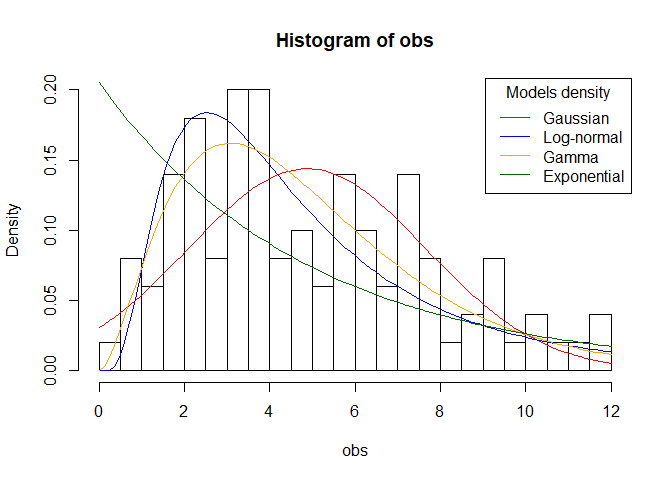
\includegraphics{practice2_files/figure-latex/unnamed-chunk-3-1.pdf}

\hypertarget{ex-3.2-estimate-the-uxfb01ve-parameters-of-the-gaussian-mixture-using-the-1000-observed-longitude-values.-you-can-done-this-numerically-in-r-with-the-optim-function.-plot-the-uxfb01tted-gaussian-mixture-on-top-of-the-histogram-of-the-longitude-data.}{%
\subsection{Ex 3.2 Estimate the five parameters of the Gaussian mixture
using the 1000 observed longitude values. You can done this numerically
in R with the optim function. Plot the fitted Gaussian mixture on top of
the histogram of the longitude
data.}\label{ex-3.2-estimate-the-uxfb01ve-parameters-of-the-gaussian-mixture-using-the-1000-observed-longitude-values.-you-can-done-this-numerically-in-r-with-the-optim-function.-plot-the-uxfb01tted-gaussian-mixture-on-top-of-the-histogram-of-the-longitude-data.}}

To obtain initial guess for the parameter of the Gaussian mixture for
the longitude locations we plot the histogram

\begin{Shaded}
\begin{Highlighting}[]
\KeywordTok{hist}\NormalTok{(quakes}\OperatorTok{$}\NormalTok{long, }\DataTypeTok{probability =} \OtherTok{TRUE}\NormalTok{, }\DataTypeTok{breaks =} \StringTok{"FD"}\NormalTok{)}
\end{Highlighting}
\end{Shaded}

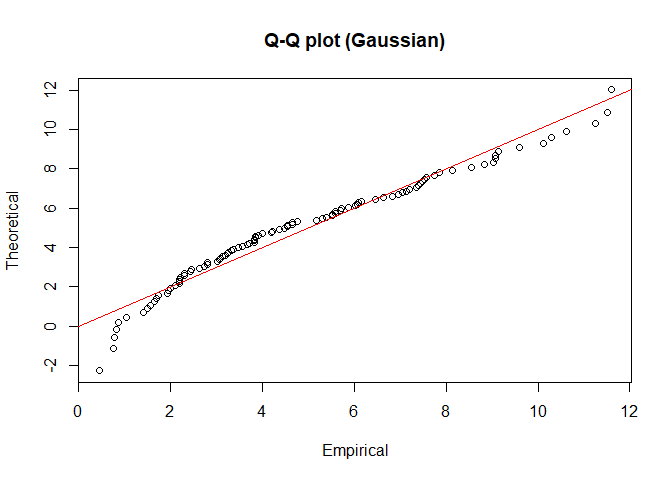
\includegraphics{practice2_files/figure-latex/unnamed-chunk-4-1.pdf}

We can divide the longitude location observations in two groups, before
and after 175.

\begin{Shaded}
\begin{Highlighting}[]
\NormalTok{before <-}\StringTok{ }\NormalTok{quakes}\OperatorTok{$}\NormalTok{long[quakes}\OperatorTok{$}\NormalTok{long }\OperatorTok{<}\StringTok{ }\DecValTok{175}\NormalTok{]}
\NormalTok{after <-}\StringTok{ }\NormalTok{quakes}\OperatorTok{$}\NormalTok{long[quakes}\OperatorTok{$}\NormalTok{long }\OperatorTok{>}\StringTok{ }\DecValTok{175}\NormalTok{]}
\end{Highlighting}
\end{Shaded}

We can now consider the following initial estimate for the Gaussian
mixture:

\begin{Shaded}
\begin{Highlighting}[]
\NormalTok{m1.init <-}\StringTok{ }\KeywordTok{mean}\NormalTok{(before)        }\CommentTok{# Or just look at the histogram and try to think what the values of}
\NormalTok{sd1.init <-}\StringTok{ }\KeywordTok{sd}\NormalTok{(before)         }\CommentTok{# the parameters can be}
\NormalTok{m2.init <-}\StringTok{ }\KeywordTok{mean}\NormalTok{(after)}
\NormalTok{sd2.init <-}\StringTok{ }\KeywordTok{sd}\NormalTok{(after)}
\NormalTok{w.init <-}\StringTok{ }\KeywordTok{length}\NormalTok{(before) }\OperatorTok{/}\StringTok{ }\KeywordTok{length}\NormalTok{(after)}
\NormalTok{par.init <-}\StringTok{ }\KeywordTok{c}\NormalTok{(m1.init, sd1.init, m2.init, sd2.init, w.init)}
\NormalTok{par.init}
\end{Highlighting}
\end{Shaded}

\begin{verbatim}
## [1] 168.2598049   1.9746871 182.3506415   2.1433270   0.2578616
\end{verbatim}

We define now the minus log-likelihood and then start the optimization

\begin{Shaded}
\begin{Highlighting}[]
\NormalTok{gaussmix_mll <-}\StringTok{ }\ControlFlowTok{function}\NormalTok{(par, data)\{}
  \ControlFlowTok{if}\NormalTok{ (par[}\DecValTok{5}\NormalTok{] }\OperatorTok{>}\StringTok{ }\DecValTok{1} \OperatorTok{||}\StringTok{ }\NormalTok{par[}\DecValTok{5}\NormalTok{] }\OperatorTok{<}\StringTok{ }\DecValTok{0}\NormalTok{ )\{}
    \KeywordTok{return}\NormalTok{(}\OtherTok{Inf}\NormalTok{)                         }\CommentTok{# why return inf?}
\NormalTok{  \}}
  \ControlFlowTok{if}\NormalTok{ (par[}\DecValTok{2}\NormalTok{] }\OperatorTok{<}\StringTok{ }\DecValTok{0} \OperatorTok{||}\StringTok{ }\NormalTok{par[}\DecValTok{4}\NormalTok{] }\OperatorTok{<}\StringTok{ }\DecValTok{0}\NormalTok{)\{}
    \KeywordTok{return}\NormalTok{(}\OtherTok{Inf}\NormalTok{)}
\NormalTok{  \}}
  \OperatorTok{-}\KeywordTok{sum}\NormalTok{(}\KeywordTok{log}\NormalTok{(}\KeywordTok{dgaussmix}\NormalTok{(}\DataTypeTok{x =}\NormalTok{ data, }\DataTypeTok{mean1 =}\NormalTok{ par[}\DecValTok{1}\NormalTok{], }\DataTypeTok{sd1 =}\NormalTok{ par[}\DecValTok{2}\NormalTok{], }
              \DataTypeTok{mean2 =}\NormalTok{ par[}\DecValTok{3}\NormalTok{], }\DataTypeTok{sd2 =}\NormalTok{ par[}\DecValTok{4}\NormalTok{], }\DataTypeTok{w =}\NormalTok{ par[}\DecValTok{5}\NormalTok{])))}
\NormalTok{\}}
\NormalTok{par.est_gaussmix <-}\StringTok{ }\KeywordTok{optim}\NormalTok{(}\DataTypeTok{f =}\NormalTok{ gaussmix_mll, }\DataTypeTok{par =}\NormalTok{ par.init, }\DataTypeTok{data =}\NormalTok{ quakes}\OperatorTok{$}\NormalTok{long)}\OperatorTok{$}\NormalTok{par}
\NormalTok{par.est_gaussmix}
\end{Highlighting}
\end{Shaded}

\begin{verbatim}
## [1] 168.236709   1.944461 182.340729   2.153245   0.204089
\end{verbatim}

I plot the density with estimated parameters.

\begin{Shaded}
\begin{Highlighting}[]
\KeywordTok{hist}\NormalTok{(quakes}\OperatorTok{$}\NormalTok{long, }\DataTypeTok{probability =} \OtherTok{TRUE}\NormalTok{, }\DataTypeTok{breaks =} \StringTok{"FD"}\NormalTok{)}
\KeywordTok{curve}\NormalTok{(}\KeywordTok{dgaussmix}\NormalTok{(x, par.est_gaussmix[}\DecValTok{1}\NormalTok{], par.est_gaussmix[}\DecValTok{2}\NormalTok{], }
\NormalTok{      par.est_gaussmix[}\DecValTok{3}\NormalTok{], par.est_gaussmix[}\DecValTok{4}\NormalTok{], par.est_gaussmix[}\DecValTok{5}\NormalTok{]), }\DataTypeTok{add =} \OtherTok{TRUE}\NormalTok{, }\DataTypeTok{col =} \StringTok{"red"}\NormalTok{)}
\end{Highlighting}
\end{Shaded}

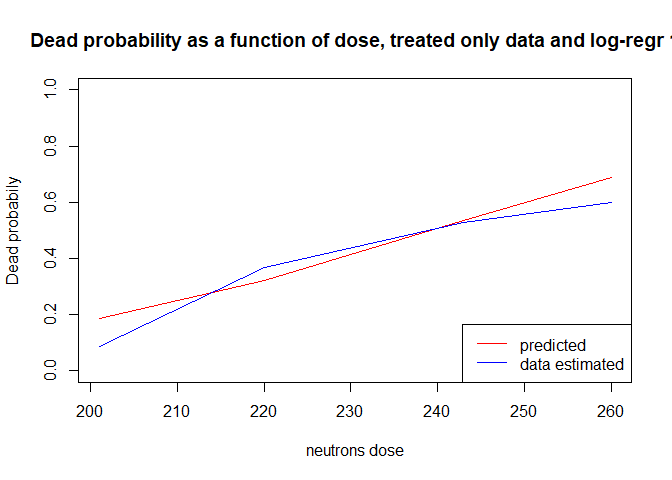
\includegraphics{practice2_files/figure-latex/unnamed-chunk-8-1.pdf}

\hypertarget{ex-3.3-consider-now-another-model-where-the-longitude-locations-are-i.i.d.-gaussian-distributed.}{%
\subsection{Ex 3.3 Consider now another model where the longitude
locations are i.i.d. Gaussian
distributed.}\label{ex-3.3-consider-now-another-model-where-the-longitude-locations-are-i.i.d.-gaussian-distributed.}}

\begin{Shaded}
\begin{Highlighting}[]
\CommentTok{# Methods of moments}
\NormalTok{mu =}\StringTok{ }\KeywordTok{mean}\NormalTok{(quakes}\OperatorTok{$}\NormalTok{long)}
\NormalTok{sigma =}\StringTok{ }\KeywordTok{sd}\NormalTok{(quakes}\OperatorTok{$}\NormalTok{long)}

\CommentTok{# Minus log likelihood}
\NormalTok{gauss_mll <-}\StringTok{ }\ControlFlowTok{function}\NormalTok{(par, data)\{}
  \OperatorTok{-}\KeywordTok{sum}\NormalTok{(}\KeywordTok{dnorm}\NormalTok{(}\DataTypeTok{x =}\NormalTok{ data, }\DataTypeTok{mean =}\NormalTok{ par[}\DecValTok{1}\NormalTok{], }\DataTypeTok{sd =}\NormalTok{ par[}\DecValTok{2}\NormalTok{]))}
\NormalTok{\} }

\NormalTok{par.est_gauss <-}\StringTok{ }\KeywordTok{optim}\NormalTok{(}\DataTypeTok{f =}\NormalTok{ gauss_mll, }\DataTypeTok{par =} \KeywordTok{c}\NormalTok{(mu, sigma),          }\CommentTok{# optim daesn't work in this the}
                 \DataTypeTok{data =}\NormalTok{ quakes}\OperatorTok{$}\NormalTok{long, }\DataTypeTok{control =} \KeywordTok{list}\NormalTok{(}\DataTypeTok{maxit =} \DecValTok{10000}\NormalTok{))}\CommentTok{# pars estimated by moments m.}
\end{Highlighting}
\end{Shaded}

\begin{verbatim}
## Warning in dnorm(x = data, mean = par[1], sd = par[2]): NaNs produced

## Warning in dnorm(x = data, mean = par[1], sd = par[2]): NaNs produced

## Warning in dnorm(x = data, mean = par[1], sd = par[2]): NaNs produced

## Warning in dnorm(x = data, mean = par[1], sd = par[2]): NaNs produced

## Warning in dnorm(x = data, mean = par[1], sd = par[2]): NaNs produced

## Warning in dnorm(x = data, mean = par[1], sd = par[2]): NaNs produced

## Warning in dnorm(x = data, mean = par[1], sd = par[2]): NaNs produced

## Warning in dnorm(x = data, mean = par[1], sd = par[2]): NaNs produced

## Warning in dnorm(x = data, mean = par[1], sd = par[2]): NaNs produced

## Warning in dnorm(x = data, mean = par[1], sd = par[2]): NaNs produced

## Warning in dnorm(x = data, mean = par[1], sd = par[2]): NaNs produced

## Warning in dnorm(x = data, mean = par[1], sd = par[2]): NaNs produced

## Warning in dnorm(x = data, mean = par[1], sd = par[2]): NaNs produced

## Warning in dnorm(x = data, mean = par[1], sd = par[2]): NaNs produced

## Warning in dnorm(x = data, mean = par[1], sd = par[2]): NaNs produced

## Warning in dnorm(x = data, mean = par[1], sd = par[2]): NaNs produced

## Warning in dnorm(x = data, mean = par[1], sd = par[2]): NaNs produced

## Warning in dnorm(x = data, mean = par[1], sd = par[2]): NaNs produced

## Warning in dnorm(x = data, mean = par[1], sd = par[2]): NaNs produced

## Warning in dnorm(x = data, mean = par[1], sd = par[2]): NaNs produced

## Warning in dnorm(x = data, mean = par[1], sd = par[2]): NaNs produced

## Warning in dnorm(x = data, mean = par[1], sd = par[2]): NaNs produced

## Warning in dnorm(x = data, mean = par[1], sd = par[2]): NaNs produced

## Warning in dnorm(x = data, mean = par[1], sd = par[2]): NaNs produced

## Warning in dnorm(x = data, mean = par[1], sd = par[2]): NaNs produced

## Warning in dnorm(x = data, mean = par[1], sd = par[2]): NaNs produced

## Warning in dnorm(x = data, mean = par[1], sd = par[2]): NaNs produced

## Warning in dnorm(x = data, mean = par[1], sd = par[2]): NaNs produced

## Warning in dnorm(x = data, mean = par[1], sd = par[2]): NaNs produced

## Warning in dnorm(x = data, mean = par[1], sd = par[2]): NaNs produced

## Warning in dnorm(x = data, mean = par[1], sd = par[2]): NaNs produced

## Warning in dnorm(x = data, mean = par[1], sd = par[2]): NaNs produced

## Warning in dnorm(x = data, mean = par[1], sd = par[2]): NaNs produced

## Warning in dnorm(x = data, mean = par[1], sd = par[2]): NaNs produced

## Warning in dnorm(x = data, mean = par[1], sd = par[2]): NaNs produced

## Warning in dnorm(x = data, mean = par[1], sd = par[2]): NaNs produced

## Warning in dnorm(x = data, mean = par[1], sd = par[2]): NaNs produced

## Warning in dnorm(x = data, mean = par[1], sd = par[2]): NaNs produced

## Warning in dnorm(x = data, mean = par[1], sd = par[2]): NaNs produced

## Warning in dnorm(x = data, mean = par[1], sd = par[2]): NaNs produced

## Warning in dnorm(x = data, mean = par[1], sd = par[2]): NaNs produced

## Warning in dnorm(x = data, mean = par[1], sd = par[2]): NaNs produced

## Warning in dnorm(x = data, mean = par[1], sd = par[2]): NaNs produced

## Warning in dnorm(x = data, mean = par[1], sd = par[2]): NaNs produced

## Warning in dnorm(x = data, mean = par[1], sd = par[2]): NaNs produced

## Warning in dnorm(x = data, mean = par[1], sd = par[2]): NaNs produced

## Warning in dnorm(x = data, mean = par[1], sd = par[2]): NaNs produced

## Warning in dnorm(x = data, mean = par[1], sd = par[2]): NaNs produced

## Warning in dnorm(x = data, mean = par[1], sd = par[2]): NaNs produced

## Warning in dnorm(x = data, mean = par[1], sd = par[2]): NaNs produced

## Warning in dnorm(x = data, mean = par[1], sd = par[2]): NaNs produced

## Warning in dnorm(x = data, mean = par[1], sd = par[2]): NaNs produced

## Warning in dnorm(x = data, mean = par[1], sd = par[2]): NaNs produced

## Warning in dnorm(x = data, mean = par[1], sd = par[2]): NaNs produced

## Warning in dnorm(x = data, mean = par[1], sd = par[2]): NaNs produced

## Warning in dnorm(x = data, mean = par[1], sd = par[2]): NaNs produced

## Warning in dnorm(x = data, mean = par[1], sd = par[2]): NaNs produced

## Warning in dnorm(x = data, mean = par[1], sd = par[2]): NaNs produced

## Warning in dnorm(x = data, mean = par[1], sd = par[2]): NaNs produced

## Warning in dnorm(x = data, mean = par[1], sd = par[2]): NaNs produced

## Warning in dnorm(x = data, mean = par[1], sd = par[2]): NaNs produced

## Warning in dnorm(x = data, mean = par[1], sd = par[2]): NaNs produced

## Warning in dnorm(x = data, mean = par[1], sd = par[2]): NaNs produced

## Warning in dnorm(x = data, mean = par[1], sd = par[2]): NaNs produced

## Warning in dnorm(x = data, mean = par[1], sd = par[2]): NaNs produced

## Warning in dnorm(x = data, mean = par[1], sd = par[2]): NaNs produced

## Warning in dnorm(x = data, mean = par[1], sd = par[2]): NaNs produced

## Warning in dnorm(x = data, mean = par[1], sd = par[2]): NaNs produced

## Warning in dnorm(x = data, mean = par[1], sd = par[2]): NaNs produced

## Warning in dnorm(x = data, mean = par[1], sd = par[2]): NaNs produced

## Warning in dnorm(x = data, mean = par[1], sd = par[2]): NaNs produced

## Warning in dnorm(x = data, mean = par[1], sd = par[2]): NaNs produced

## Warning in dnorm(x = data, mean = par[1], sd = par[2]): NaNs produced
\end{verbatim}

\begin{Shaded}
\begin{Highlighting}[]
\KeywordTok{hist}\NormalTok{(quakes}\OperatorTok{$}\NormalTok{long, }\DataTypeTok{probability =} \OtherTok{TRUE}\NormalTok{, }\DataTypeTok{breaks =} \StringTok{"FD"}\NormalTok{)}
\KeywordTok{curve}\NormalTok{(}\KeywordTok{dnorm}\NormalTok{(x, }\DataTypeTok{mean =}\NormalTok{ mu, }\DataTypeTok{sd =}\NormalTok{ sigma), }\DataTypeTok{add =} \OtherTok{TRUE}\NormalTok{, }\DataTypeTok{col =} \StringTok{"red"}\NormalTok{)}
\end{Highlighting}
\end{Shaded}

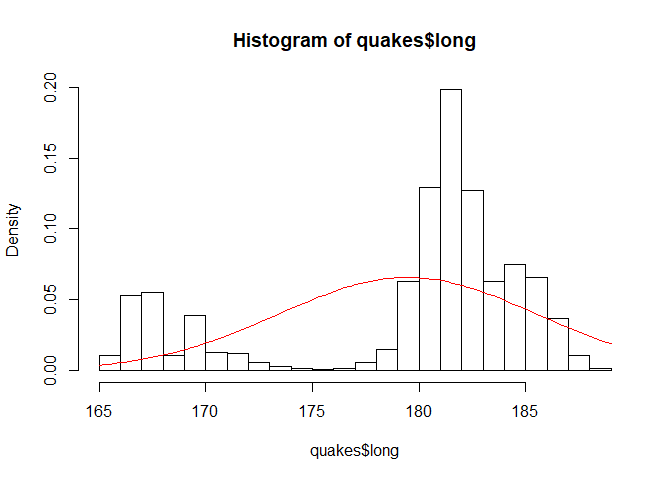
\includegraphics{practice2_files/figure-latex/unnamed-chunk-10-1.pdf}

\hypertarget{ex-3.4-compute-the-aic-and-bic-values-for-the-simple-gaussian-model-and-the-gaussian-mixture-model-for-the-longitude-data.-which-model-should-be-selected}{%
\subsection{Ex 3.4 Compute the AIC and BIC values for the simple
Gaussian model and the Gaussian mixture model for the longitude data.
Which model should be
selected?}\label{ex-3.4-compute-the-aic-and-bic-values-for-the-simple-gaussian-model-and-the-gaussian-mixture-model-for-the-longitude-data.-which-model-should-be-selected}}

\begin{Shaded}
\begin{Highlighting}[]
\NormalTok{mll.mixture <-}\StringTok{ }\KeywordTok{gaussmix_mll}\NormalTok{(}\DataTypeTok{data =}\NormalTok{ quakes}\OperatorTok{$}\NormalTok{long, }\DataTypeTok{par =}\NormalTok{ par.est_gaussmix)}
\NormalTok{mll.gauss <-}\StringTok{ }\NormalTok{(}\OperatorTok{-}\KeywordTok{sum}\NormalTok{(}\KeywordTok{dnorm}\NormalTok{(}\DataTypeTok{x =}\NormalTok{ quakes}\OperatorTok{$}\NormalTok{long, }\DataTypeTok{mean =}\NormalTok{ mu, }\DataTypeTok{sd =}\NormalTok{ sigma, }\DataTypeTok{log =} \OtherTok{TRUE}\NormalTok{)))}

\CommentTok{# AIC}
\NormalTok{aic.mixture <-}\StringTok{ }\DecValTok{2} \OperatorTok{*}\StringTok{ }\NormalTok{mll.mixture }\OperatorTok{+}\StringTok{ }\DecValTok{2} \OperatorTok{*}\StringTok{ }\KeywordTok{length}\NormalTok{(par.est_gaussmix)}
\NormalTok{aic.gauss <-}\StringTok{ }\DecValTok{2} \OperatorTok{*}\StringTok{ }\NormalTok{mll.gauss }\OperatorTok{+}\StringTok{ }\DecValTok{2} \OperatorTok{*}\StringTok{ }\DecValTok{2}
\KeywordTok{c}\NormalTok{(aic.mixture, aic.gauss)}
\end{Highlighting}
\end{Shaded}

\begin{verbatim}
## [1] 5349.808 6447.428
\end{verbatim}

\begin{Shaded}
\begin{Highlighting}[]
\CommentTok{# BIC}
\NormalTok{n <-}\StringTok{ }\KeywordTok{nrow}\NormalTok{(quakes)}
\NormalTok{bic.mixture <-}\StringTok{ }\DecValTok{2} \OperatorTok{*}\StringTok{ }\NormalTok{mll.mixture }\OperatorTok{+}\StringTok{ }\KeywordTok{length}\NormalTok{(par.est_gaussmix) }\OperatorTok{*}\StringTok{ }\KeywordTok{log}\NormalTok{(n)}
\NormalTok{bic.gauss <-}\StringTok{ }\DecValTok{2} \OperatorTok{*}\StringTok{ }\NormalTok{mll.gauss }\OperatorTok{+}\StringTok{ }\DecValTok{2} \OperatorTok{*}\StringTok{ }\KeywordTok{log}\NormalTok{(n)}
\KeywordTok{c}\NormalTok{(}\DataTypeTok{mixture =}\NormalTok{ bic.mixture, }\DataTypeTok{gauss =}\NormalTok{ bic.gauss)}
\end{Highlighting}
\end{Shaded}

\begin{verbatim}
##  mixture    gauss 
## 5374.347 6457.244
\end{verbatim}

BIC and AIC scores indicates that the mixture model should be selected.

\hypertarget{ex-3.5-repeat-the-above-uxfb01tting-procedure-for-the-latitude-and-the-depth-data-and-perform-as-usual-model-selection-using-aic-and-bic-which-model-should-be-used}{%
\subsection{Ex 3.5 Repeat the above fitting procedure for the latitude
and the depth data, and perform as usual model selection using AIC and
BIC, which model should be
used?}\label{ex-3.5-repeat-the-above-uxfb01tting-procedure-for-the-latitude-and-the-depth-data-and-perform-as-usual-model-selection-using-aic-and-bic-which-model-should-be-used}}

\hypertarget{latitude-data-fit}{%
\subsubsection{Latitude data fit}\label{latitude-data-fit}}

\begin{Shaded}
\begin{Highlighting}[]
\KeywordTok{hist}\NormalTok{(quakes}\OperatorTok{$}\NormalTok{lat, }\DataTypeTok{probability =} \OtherTok{TRUE}\NormalTok{, }\DataTypeTok{breaks =} \StringTok{"FD"}\NormalTok{)}
\end{Highlighting}
\end{Shaded}

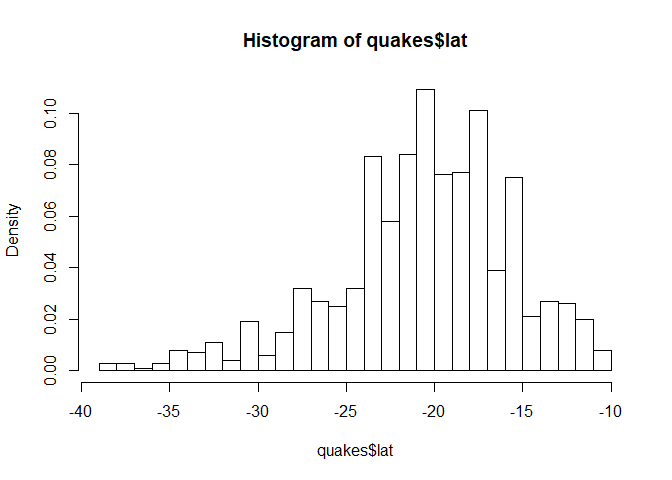
\includegraphics{practice2_files/figure-latex/unnamed-chunk-12-1.pdf}

\begin{Shaded}
\begin{Highlighting}[]
\CommentTok{# Parameters mixture}
\NormalTok{par.lat <-}\StringTok{ }\KeywordTok{optim}\NormalTok{(}\DataTypeTok{par =} \KeywordTok{c}\NormalTok{(}\OperatorTok{-}\DecValTok{32}\NormalTok{, }\DecValTok{7}\NormalTok{, }\DecValTok{-20}\NormalTok{, }\DecValTok{7}\NormalTok{, }\FloatTok{0.5}\NormalTok{), }\DataTypeTok{fn =}\NormalTok{ gaussmix_mll, }\DataTypeTok{data =}\NormalTok{ quakes}\OperatorTok{$}\NormalTok{lat)}\OperatorTok{$}\NormalTok{par}

\CommentTok{# Parameters gauss}
\NormalTok{mu.lat <-}\StringTok{ }\KeywordTok{mean}\NormalTok{(quakes}\OperatorTok{$}\NormalTok{lat)}
\NormalTok{sigma.lat <-}\StringTok{ }\KeywordTok{sd}\NormalTok{(quakes}\OperatorTok{$}\NormalTok{lat)}

\KeywordTok{hist}\NormalTok{(quakes}\OperatorTok{$}\NormalTok{lat, }\DataTypeTok{probability =} \OtherTok{TRUE}\NormalTok{, }\DataTypeTok{breaks =} \StringTok{"FD"}\NormalTok{)}
\KeywordTok{curve}\NormalTok{(}\KeywordTok{dgaussmix}\NormalTok{(x, par.lat[}\DecValTok{1}\NormalTok{], par.lat[}\DecValTok{2}\NormalTok{], par.lat[}\DecValTok{3}\NormalTok{], par.lat[}\DecValTok{4}\NormalTok{], par.lat[}\DecValTok{5}\NormalTok{]), }
                \DataTypeTok{add =} \OtherTok{TRUE}\NormalTok{, }\DataTypeTok{col =} \StringTok{"red"}\NormalTok{)}
\KeywordTok{curve}\NormalTok{(}\KeywordTok{dnorm}\NormalTok{(x, }\DataTypeTok{mean =}\NormalTok{ mu.lat, }\DataTypeTok{sd =}\NormalTok{ sigma.lat), }\DataTypeTok{col =} \StringTok{"blue"}\NormalTok{, }\DataTypeTok{add =} \OtherTok{TRUE}\NormalTok{)}
\KeywordTok{legend}\NormalTok{(}\StringTok{"topleft"}\NormalTok{, }\DataTypeTok{legend =} \KeywordTok{c}\NormalTok{(}\StringTok{"mixture"}\NormalTok{, }\StringTok{"gaussian"}\NormalTok{), }\DataTypeTok{col =} \KeywordTok{c}\NormalTok{(}\StringTok{"red"}\NormalTok{, }\StringTok{"blue"}\NormalTok{), }\DataTypeTok{lty =} \DecValTok{1}\NormalTok{)}
\end{Highlighting}
\end{Shaded}

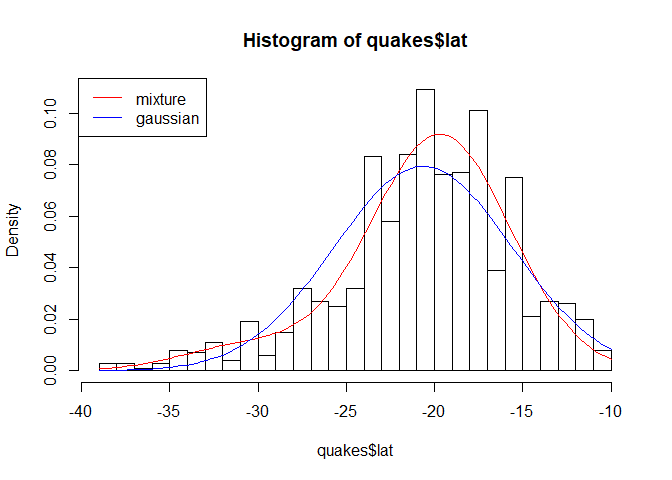
\includegraphics{practice2_files/figure-latex/unnamed-chunk-13-1.pdf}

\begin{Shaded}
\begin{Highlighting}[]
\NormalTok{mll.mixture =}\StringTok{ }\KeywordTok{gaussmix_mll}\NormalTok{(par.lat, }\DataTypeTok{data =}\NormalTok{ quakes}\OperatorTok{$}\NormalTok{lat)}
\NormalTok{mll.gauss =}\StringTok{ }\OperatorTok{-}\KeywordTok{sum}\NormalTok{(}\KeywordTok{dnorm}\NormalTok{(quakes}\OperatorTok{$}\NormalTok{lat, mu.lat, sigma.lat, }\DataTypeTok{log =} \OtherTok{TRUE}\NormalTok{))}

\CommentTok{# AIC}
\NormalTok{aic.mixture <-}\StringTok{ }\DecValTok{2} \OperatorTok{*}\StringTok{ }\NormalTok{mll.mixture }\OperatorTok{+}\StringTok{ }\DecValTok{2} \OperatorTok{*}\StringTok{ }\KeywordTok{length}\NormalTok{(par.lat)}
\NormalTok{aic.gauss <-}\StringTok{ }\DecValTok{2} \OperatorTok{*}\StringTok{ }\NormalTok{mll.gauss }\OperatorTok{+}\StringTok{ }\DecValTok{2} \OperatorTok{*}\StringTok{ }\DecValTok{2}
\KeywordTok{c}\NormalTok{(}\DataTypeTok{mixture =}\NormalTok{ aic.mixture, }\DataTypeTok{gauss =}\NormalTok{ aic.gauss)}
\end{Highlighting}
\end{Shaded}

\begin{verbatim}
##  mixture    gauss 
## 5995.310 6071.236
\end{verbatim}

\begin{Shaded}
\begin{Highlighting}[]
\CommentTok{# BIC}
\NormalTok{n =}\StringTok{ }\KeywordTok{nrow}\NormalTok{(quakes)}
\NormalTok{bic.mixture <-}\StringTok{ }\DecValTok{2} \OperatorTok{*}\StringTok{ }\NormalTok{mll.mixture }\OperatorTok{+}\StringTok{ }\KeywordTok{length}\NormalTok{(par.lat) }\OperatorTok{*}\StringTok{ }\KeywordTok{log}\NormalTok{(n)}
\NormalTok{bic.gauss <-}\StringTok{ }\DecValTok{2} \OperatorTok{*}\StringTok{ }\NormalTok{mll.gauss }\OperatorTok{+}\StringTok{ }\DecValTok{2} \OperatorTok{*}\StringTok{ }\KeywordTok{log}\NormalTok{(n)}
\KeywordTok{c}\NormalTok{(}\DataTypeTok{mixture =}\NormalTok{ bic.mixture, }\DataTypeTok{gauss =}\NormalTok{ bic.gauss)}
\end{Highlighting}
\end{Shaded}

\begin{verbatim}
##  mixture    gauss 
## 6019.848 6081.052
\end{verbatim}

The mixture model is to prefer (AIC and BIC).

\hypertarget{latitude-data-fit-1}{%
\subsubsection{Latitude data fit}\label{latitude-data-fit-1}}

\begin{Shaded}
\begin{Highlighting}[]
\KeywordTok{hist}\NormalTok{(quakes}\OperatorTok{$}\NormalTok{depth, }\DataTypeTok{probability =} \OtherTok{TRUE}\NormalTok{, }\DataTypeTok{breaks =} \DecValTok{30}\NormalTok{)}
\end{Highlighting}
\end{Shaded}

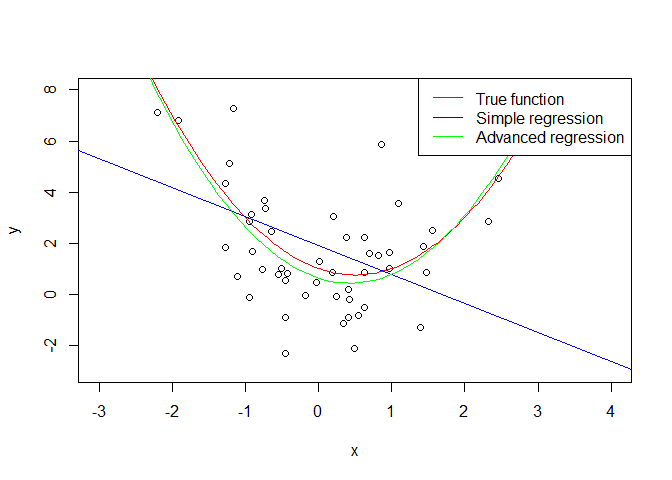
\includegraphics{practice2_files/figure-latex/unnamed-chunk-15-1.pdf}

\begin{Shaded}
\begin{Highlighting}[]
\CommentTok{# Parameters mixture}
\NormalTok{par.depth <-}\StringTok{ }\KeywordTok{optim}\NormalTok{(}\DataTypeTok{par =} \KeywordTok{c}\NormalTok{(}\DecValTok{110}\NormalTok{, }\DecValTok{100}\NormalTok{, }\DecValTok{600}\NormalTok{, }\DecValTok{100}\NormalTok{, }\FloatTok{0.5}\NormalTok{), }\DataTypeTok{fn =}\NormalTok{ gaussmix_mll, }\DataTypeTok{data =}\NormalTok{ quakes}\OperatorTok{$}\NormalTok{depth)}\OperatorTok{$}\NormalTok{par}

\CommentTok{# Parameters gauss}
\NormalTok{mu.depth <-}\StringTok{ }\KeywordTok{mean}\NormalTok{(quakes}\OperatorTok{$}\NormalTok{depth)}
\NormalTok{sigma.depth <-}\StringTok{ }\KeywordTok{sd}\NormalTok{(quakes}\OperatorTok{$}\NormalTok{depth)}

\KeywordTok{hist}\NormalTok{(quakes}\OperatorTok{$}\NormalTok{depth, }\DataTypeTok{probability =} \OtherTok{TRUE}\NormalTok{, }\DataTypeTok{breaks =} \DecValTok{30}\NormalTok{)}
\KeywordTok{curve}\NormalTok{(}\KeywordTok{dgaussmix}\NormalTok{(x, par.depth[}\DecValTok{1}\NormalTok{], par.depth[}\DecValTok{2}\NormalTok{], par.depth[}\DecValTok{3}\NormalTok{], par.depth[}\DecValTok{4}\NormalTok{], par.depth[}\DecValTok{5}\NormalTok{]), }
                \DataTypeTok{add =} \OtherTok{TRUE}\NormalTok{, }\DataTypeTok{col =} \StringTok{"red"}\NormalTok{)}
\KeywordTok{curve}\NormalTok{(}\KeywordTok{dnorm}\NormalTok{(x, }\DataTypeTok{mean =}\NormalTok{ mu.depth, }\DataTypeTok{sd =}\NormalTok{ sigma.depth), }\DataTypeTok{col =} \StringTok{"blue"}\NormalTok{, }\DataTypeTok{add =} \OtherTok{TRUE}\NormalTok{)}
\KeywordTok{legend}\NormalTok{(}\StringTok{"topleft"}\NormalTok{, }\DataTypeTok{legend =} \KeywordTok{c}\NormalTok{(}\StringTok{"mixture"}\NormalTok{, }\StringTok{"gaussian"}\NormalTok{), }\DataTypeTok{col =} \KeywordTok{c}\NormalTok{(}\StringTok{"red"}\NormalTok{, }\StringTok{"blue"}\NormalTok{), }\DataTypeTok{lty =} \DecValTok{1}\NormalTok{)}
\end{Highlighting}
\end{Shaded}

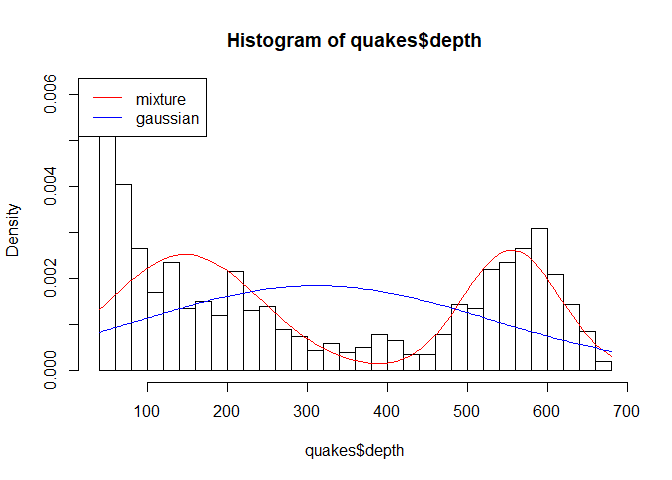
\includegraphics{practice2_files/figure-latex/unnamed-chunk-16-1.pdf}

\begin{Shaded}
\begin{Highlighting}[]
\NormalTok{mll.mixture =}\StringTok{ }\KeywordTok{gaussmix_mll}\NormalTok{(par.depth, }\DataTypeTok{data =}\NormalTok{ quakes}\OperatorTok{$}\NormalTok{depth)}
\NormalTok{mll.gauss =}\StringTok{ }\OperatorTok{-}\KeywordTok{sum}\NormalTok{(}\KeywordTok{dnorm}\NormalTok{(quakes}\OperatorTok{$}\NormalTok{depth, mu.depth, sigma.depth, }\DataTypeTok{log =} \OtherTok{TRUE}\NormalTok{))}

\CommentTok{# AIC}
\NormalTok{aic.mixture <-}\StringTok{ }\DecValTok{2} \OperatorTok{*}\StringTok{ }\NormalTok{mll.mixture }\OperatorTok{+}\StringTok{ }\DecValTok{2} \OperatorTok{*}\StringTok{ }\KeywordTok{length}\NormalTok{(par.depth)}
\NormalTok{aic.gauss <-}\StringTok{ }\DecValTok{2} \OperatorTok{*}\StringTok{ }\NormalTok{mll.gauss }\OperatorTok{+}\StringTok{ }\DecValTok{2} \OperatorTok{*}\StringTok{ }\DecValTok{2}
\KeywordTok{c}\NormalTok{(}\DataTypeTok{mixture =}\NormalTok{ aic.mixture, }\DataTypeTok{gauss =}\NormalTok{ aic.gauss)}
\end{Highlighting}
\end{Shaded}

\begin{verbatim}
##  mixture    gauss 
## 12903.48 13587.13
\end{verbatim}

\begin{Shaded}
\begin{Highlighting}[]
\CommentTok{# BIC}
\NormalTok{n =}\StringTok{ }\KeywordTok{nrow}\NormalTok{(quakes)}
\NormalTok{bic.mixture <-}\StringTok{ }\DecValTok{2} \OperatorTok{*}\StringTok{ }\NormalTok{mll.mixture }\OperatorTok{+}\StringTok{ }\KeywordTok{length}\NormalTok{(par.lat) }\OperatorTok{*}\StringTok{ }\KeywordTok{log}\NormalTok{(n)}
\NormalTok{bic.gauss <-}\StringTok{ }\DecValTok{2} \OperatorTok{*}\StringTok{ }\NormalTok{mll.gauss }\OperatorTok{+}\StringTok{ }\DecValTok{2} \OperatorTok{*}\StringTok{ }\KeywordTok{log}\NormalTok{(n)}
\KeywordTok{c}\NormalTok{(}\DataTypeTok{mixture =}\NormalTok{ bic.mixture, }\DataTypeTok{gauss =}\NormalTok{ bic.gauss)}
\end{Highlighting}
\end{Shaded}

\begin{verbatim}
##  mixture    gauss 
## 12928.02 13596.94
\end{verbatim}

\hypertarget{in-this-question-we-consider-a-generalized-linear-model-with-the-log-link-and-stations-follows-a-gaussian-distribution.}{%
\subsection{3.6 In this question we consider a generalized linear model
with the log link and stations follows a Gaussian
distribution.}\label{in-this-question-we-consider-a-generalized-linear-model-with-the-log-link-and-stations-follows-a-gaussian-distribution.}}

\begin{Shaded}
\begin{Highlighting}[]
\NormalTok{fit1 <-}\StringTok{ }\KeywordTok{glm}\NormalTok{(stations }\OperatorTok{~}\StringTok{ }\NormalTok{., }\DataTypeTok{data =}\NormalTok{ quakes, }\DataTypeTok{family =} \KeywordTok{gaussian}\NormalTok{(}\DataTypeTok{link =} \StringTok{"log"}\NormalTok{))}
\KeywordTok{summary}\NormalTok{(fit1)}
\end{Highlighting}
\end{Shaded}

\begin{verbatim}
## 
## Call:
## glm(formula = stations ~ ., family = gaussian(link = "log"), 
##     data = quakes)
## 
## Deviance Residuals: 
##     Min       1Q   Median       3Q      Max  
## -67.512   -6.380   -1.474    4.391   46.943  
## 
## Coefficients:
##               Estimate Std. Error t value Pr(>|t|)    
## (Intercept) -4.2425771  0.2908656 -14.586  < 2e-16 ***
## lat          0.0079305  0.0018178   4.363 1.42e-05 ***
## long         0.0140097  0.0014976   9.355  < 2e-16 ***
## depth        0.0002845  0.0000392   7.257 7.94e-13 ***
## mag          1.1290611  0.0170562  66.197  < 2e-16 ***
## ---
## Signif. codes:  0 '***' 0.001 '**' 0.01 '*' 0.05 '.' 0.1 ' ' 1
## 
## (Dispersion parameter for gaussian family taken to be 107.1978)
## 
##     Null deviance: 479147  on 999  degrees of freedom
## Residual deviance: 106661  on 995  degrees of freedom
## AIC: 7519.5
## 
## Number of Fisher Scoring iterations: 5
\end{verbatim}

\begin{Shaded}
\begin{Highlighting}[]
\NormalTok{fit2 <-}\StringTok{ }\KeywordTok{glm}\NormalTok{(stations }\OperatorTok{~}\StringTok{ }\NormalTok{. }\OperatorTok{+}\StringTok{ }\KeywordTok{I}\NormalTok{(mag}\OperatorTok{^}\DecValTok{2}\NormalTok{), }\DataTypeTok{data =}\NormalTok{ quakes, }\DataTypeTok{family =} \KeywordTok{gaussian}\NormalTok{(}\DataTypeTok{link =} \StringTok{"log"}\NormalTok{))}
\KeywordTok{summary}\NormalTok{(fit2)}
\end{Highlighting}
\end{Shaded}

\begin{verbatim}
## 
## Call:
## glm(formula = stations ~ . + I(mag^2), family = gaussian(link = "log"), 
##     data = quakes)
## 
## Deviance Residuals: 
##     Min       1Q   Median       3Q      Max  
## -43.310   -5.327   -0.270    5.469   42.920  
## 
## Coefficients:
##               Estimate Std. Error t value Pr(>|t|)    
## (Intercept) -1.159e+01  7.478e-01 -15.501  < 2e-16 ***
## lat          9.271e-03  1.693e-03   5.475 5.53e-08 ***
## long         1.098e-02  1.391e-03   7.893 7.79e-15 ***
## depth        2.904e-04  3.628e-05   8.005 3.33e-15 ***
## mag          4.233e+00  2.891e-01  14.642  < 2e-16 ***
## I(mag^2)    -3.013e-01  2.811e-02 -10.716  < 2e-16 ***
## ---
## Signif. codes:  0 '***' 0.001 '**' 0.01 '*' 0.05 '.' 0.1 ' ' 1
## 
## (Dispersion parameter for gaussian family taken to be 94.54226)
## 
##     Null deviance: 479147  on 999  degrees of freedom
## Residual deviance:  93974  on 994  degrees of freedom
## AIC: 7394.9
## 
## Number of Fisher Scoring iterations: 5
\end{verbatim}

\begin{Shaded}
\begin{Highlighting}[]
\NormalTok{fit3 <-}\StringTok{ }\KeywordTok{glm}\NormalTok{(stations }\OperatorTok{~}\StringTok{ }\NormalTok{. }\OperatorTok{+}\StringTok{ }\KeywordTok{I}\NormalTok{(mag}\OperatorTok{^}\DecValTok{2}\NormalTok{), }\DataTypeTok{data =}\NormalTok{ quakes, }\DataTypeTok{family =} \KeywordTok{gaussian}\NormalTok{(}\DataTypeTok{link =} \StringTok{"log"}\NormalTok{))}
\KeywordTok{summary}\NormalTok{(fit2)}
\end{Highlighting}
\end{Shaded}

\begin{verbatim}
## 
## Call:
## glm(formula = stations ~ . + I(mag^2), family = gaussian(link = "log"), 
##     data = quakes)
## 
## Deviance Residuals: 
##     Min       1Q   Median       3Q      Max  
## -43.310   -5.327   -0.270    5.469   42.920  
## 
## Coefficients:
##               Estimate Std. Error t value Pr(>|t|)    
## (Intercept) -1.159e+01  7.478e-01 -15.501  < 2e-16 ***
## lat          9.271e-03  1.693e-03   5.475 5.53e-08 ***
## long         1.098e-02  1.391e-03   7.893 7.79e-15 ***
## depth        2.904e-04  3.628e-05   8.005 3.33e-15 ***
## mag          4.233e+00  2.891e-01  14.642  < 2e-16 ***
## I(mag^2)    -3.013e-01  2.811e-02 -10.716  < 2e-16 ***
## ---
## Signif. codes:  0 '***' 0.001 '**' 0.01 '*' 0.05 '.' 0.1 ' ' 1
## 
## (Dispersion parameter for gaussian family taken to be 94.54226)
## 
##     Null deviance: 479147  on 999  degrees of freedom
## Residual deviance:  93974  on 994  degrees of freedom
## AIC: 7394.9
## 
## Number of Fisher Scoring iterations: 5
\end{verbatim}

\begin{Shaded}
\begin{Highlighting}[]
\NormalTok{fit3 <-}\StringTok{ }\KeywordTok{glm}\NormalTok{(stations }\OperatorTok{~}\StringTok{ }\NormalTok{lat }\OperatorTok{+}\StringTok{ }\NormalTok{long }\OperatorTok{+}\StringTok{ }\NormalTok{depth }\OperatorTok{+}\StringTok{ }\KeywordTok{exp}\NormalTok{(mag) }\OperatorTok{+}\StringTok{ }
\StringTok{              }\KeywordTok{I}\NormalTok{(}\KeywordTok{exp}\NormalTok{(mag)}\OperatorTok{^}\DecValTok{2}\NormalTok{), }\DataTypeTok{data =}\NormalTok{ quakes, }\DataTypeTok{family =} \KeywordTok{gaussian}\NormalTok{(}\DataTypeTok{link =} \StringTok{"log"}\NormalTok{))}
\KeywordTok{summary}\NormalTok{(fit3)}
\end{Highlighting}
\end{Shaded}

\begin{verbatim}
## 
## Call:
## glm(formula = stations ~ lat + long + depth + exp(mag) + I(exp(mag)^2), 
##     family = gaussian(link = "log"), data = quakes)
## 
## Deviance Residuals: 
##     Min       1Q   Median       3Q      Max  
## -45.060   -6.508   -1.353    4.451   77.861  
## 
## Coefficients:
##                 Estimate Std. Error t value Pr(>|t|)    
## (Intercept)    6.818e-01  2.529e-01   2.696  0.00713 ** 
## lat            9.407e-03  1.768e-03   5.322 1.27e-07 ***
## long           8.423e-03  1.470e-03   5.731 1.32e-08 ***
## depth          2.534e-04  3.837e-05   6.605 6.48e-11 ***
## exp(mag)       1.465e-02  3.701e-04  39.577  < 2e-16 ***
## I(exp(mag)^2) -1.935e-05  8.130e-07 -23.796  < 2e-16 ***
## ---
## Signif. codes:  0 '***' 0.001 '**' 0.01 '*' 0.05 '.' 0.1 ' ' 1
## 
## (Dispersion parameter for gaussian family taken to be 104.8708)
## 
##     Null deviance: 479147  on 999  degrees of freedom
## Residual deviance: 104240  on 994  degrees of freedom
## AIC: 7498.6
## 
## Number of Fisher Scoring iterations: 11
\end{verbatim}

\hypertarget{ex-3.7-perform-the-log-likelihood-ratio-test-selection-between-model-1-and-model-2.}{%
\subsection{Ex 3.7 Perform the log likelihood ratio test selection
between model 1 and model
2.}\label{ex-3.7-perform-the-log-likelihood-ratio-test-selection-between-model-1-and-model-2.}}

\begin{Shaded}
\begin{Highlighting}[]
\KeywordTok{anova}\NormalTok{(fit1, fit2, }\DataTypeTok{test =} \StringTok{"LRT"}\NormalTok{)}
\end{Highlighting}
\end{Shaded}

\begin{verbatim}
## Analysis of Deviance Table
## 
## Model 1: stations ~ lat + long + depth + mag
## Model 2: stations ~ lat + long + depth + mag + I(mag^2)
##   Resid. Df Resid. Dev Df Deviance  Pr(>Chi)    
## 1       995     106661                          
## 2       994      93974  1    12688 < 2.2e-16 ***
## ---
## Signif. codes:  0 '***' 0.001 '**' 0.01 '*' 0.05 '.' 0.1 ' ' 1
\end{verbatim}

The p-value is very small and we thus reject the null hypothesis
(e.g.~at a level 0.0005) that the simpler model fit1 is sufficient.

\hypertarget{use-instead-aic-and-bic-to-perform-model-selection-between-model-1-model-2-and-model-3.}{%
\subsubsection{Use instead AIC and BIC to perform model selection
between model 1, model 2 and model
3.}\label{use-instead-aic-and-bic-to-perform-model-selection-between-model-1-model-2-and-model-3.}}

\begin{Shaded}
\begin{Highlighting}[]
\NormalTok{models <-}\StringTok{ }\KeywordTok{list}\NormalTok{(}\DataTypeTok{fit1 =}\NormalTok{ fit1, }\DataTypeTok{fit2 =}\NormalTok{ fit2, }\DataTypeTok{fit3 =}\NormalTok{ fit3)}
\KeywordTok{sapply}\NormalTok{(models, }\ControlFlowTok{function}\NormalTok{(m)\{}
  \KeywordTok{c}\NormalTok{(}\DataTypeTok{AIC =} \KeywordTok{AIC}\NormalTok{(m), }\DataTypeTok{BIC =} \KeywordTok{BIC}\NormalTok{(m))}
\NormalTok{\})}
\end{Highlighting}
\end{Shaded}

\begin{verbatim}
##         fit1     fit2     fit3
## AIC 7519.536 7394.894 7498.570
## BIC 7548.983 7429.248 7532.924
\end{verbatim}

\begin{Shaded}
\begin{Highlighting}[]
\KeywordTok{AIC}\NormalTok{(fit1, fit2, fit3)}
\end{Highlighting}
\end{Shaded}

\begin{verbatim}
##      df      AIC
## fit1  6 7519.536
## fit2  7 7394.894
## fit3  7 7498.570
\end{verbatim}

\begin{Shaded}
\begin{Highlighting}[]
\KeywordTok{BIC}\NormalTok{(fit1, fit2, fit3)}
\end{Highlighting}
\end{Shaded}

\begin{verbatim}
##      df      BIC
## fit1  6 7548.983
## fit2  7 7429.248
## fit3  7 7532.924
\end{verbatim}

Model 2 is selected by both AIC and BIC.

\hypertarget{fit-the-poisson-regression-models-with-the-log-link-function.}{%
\subsection{3.8 Fit the Poisson regression models with the log link
function.}\label{fit-the-poisson-regression-models-with-the-log-link-function.}}

\begin{Shaded}
\begin{Highlighting}[]
\NormalTok{fit4 <-}\StringTok{ }\KeywordTok{glm}\NormalTok{(stations }\OperatorTok{~}\StringTok{ }\NormalTok{., }\DataTypeTok{data =}\NormalTok{ quakes, }\DataTypeTok{family =} \KeywordTok{poisson}\NormalTok{(}\DataTypeTok{link =} \StringTok{"log"}\NormalTok{))}
\KeywordTok{summary}\NormalTok{(fit4)}
\end{Highlighting}
\end{Shaded}

\begin{verbatim}
## 
## Call:
## glm(formula = stations ~ ., family = poisson(link = "log"), data = quakes)
## 
## Deviance Residuals: 
##     Min       1Q   Median       3Q      Max  
## -7.3543  -1.1201  -0.1238   0.9457   5.9071  
## 
## Coefficients:
##               Estimate Std. Error z value Pr(>|z|)    
## (Intercept) -3.9057762  0.1848110 -21.134  < 2e-16 ***
## lat          0.0068245  0.0011614   5.876  4.2e-09 ***
## long         0.0098097  0.0009717  10.095  < 2e-16 ***
## depth        0.0002722  0.0000257  10.591  < 2e-16 ***
## mag          1.2088383  0.0118700 101.840  < 2e-16 ***
## ---
## Signif. codes:  0 '***' 0.001 '**' 0.01 '*' 0.05 '.' 0.1 ' ' 1
## 
## (Dispersion parameter for poisson family taken to be 1)
## 
##     Null deviance: 12198.5  on 999  degrees of freedom
## Residual deviance:  2764.3  on 995  degrees of freedom
## AIC: 7950.4
## 
## Number of Fisher Scoring iterations: 4
\end{verbatim}

\begin{Shaded}
\begin{Highlighting}[]
\NormalTok{fit5 <-}\StringTok{ }\KeywordTok{glm}\NormalTok{(stations }\OperatorTok{~}\StringTok{ }\NormalTok{. }\OperatorTok{+}\StringTok{ }\KeywordTok{I}\NormalTok{(mag}\OperatorTok{^}\DecValTok{2}\NormalTok{), }\DataTypeTok{data =}\NormalTok{ quakes, }
            \DataTypeTok{family =} \KeywordTok{poisson}\NormalTok{(}\DataTypeTok{link =} \StringTok{"log"}\NormalTok{))}
\KeywordTok{summary}\NormalTok{(fit5)}
\end{Highlighting}
\end{Shaded}

\begin{verbatim}
## 
## Call:
## glm(formula = stations ~ . + I(mag^2), family = poisson(link = "log"), 
##     data = quakes)
## 
## Deviance Residuals: 
##     Min       1Q   Median       3Q      Max  
## -6.6110  -1.0989  -0.0992   0.9355   5.9666  
## 
## Coefficients:
##               Estimate Std. Error z value Pr(>|z|)    
## (Intercept) -8.774e+00  5.158e-01 -17.011  < 2e-16 ***
## lat          7.597e-03  1.163e-03   6.529 6.61e-11 ***
## long         9.576e-03  9.686e-04   9.887  < 2e-16 ***
## depth        2.868e-04  2.565e-05  11.180  < 2e-16 ***
## mag          3.209e+00  1.979e-01  16.216  < 2e-16 ***
## I(mag^2)    -2.014e-01  1.991e-02 -10.113  < 2e-16 ***
## ---
## Signif. codes:  0 '***' 0.001 '**' 0.01 '*' 0.05 '.' 0.1 ' ' 1
## 
## (Dispersion parameter for poisson family taken to be 1)
## 
##     Null deviance: 12198.5  on 999  degrees of freedom
## Residual deviance:  2657.2  on 994  degrees of freedom
## AIC: 7845.3
## 
## Number of Fisher Scoring iterations: 4
\end{verbatim}

\begin{Shaded}
\begin{Highlighting}[]
\NormalTok{fit6 <-}\StringTok{ }\KeywordTok{glm}\NormalTok{(stations }\OperatorTok{~}\StringTok{ }\NormalTok{lat }\OperatorTok{+}\StringTok{ }\NormalTok{long }\OperatorTok{+}\StringTok{ }\NormalTok{depth }\OperatorTok{+}\StringTok{ }\KeywordTok{exp}\NormalTok{(mag) }\OperatorTok{+}\StringTok{ }\KeywordTok{I}\NormalTok{(}\KeywordTok{exp}\NormalTok{(mag)}\OperatorTok{^}\DecValTok{2}\NormalTok{), }
            \DataTypeTok{data =}\NormalTok{ quakes, }\DataTypeTok{family =} \KeywordTok{poisson}\NormalTok{(}\DataTypeTok{link =} \StringTok{"log"}\NormalTok{))}
\KeywordTok{summary}\NormalTok{(fit6)}
\end{Highlighting}
\end{Shaded}

\begin{verbatim}
## 
## Call:
## glm(formula = stations ~ lat + long + depth + exp(mag) + I(exp(mag)^2), 
##     family = poisson(link = "log"), data = quakes)
## 
## Deviance Residuals: 
##     Min       1Q   Median       3Q      Max  
## -7.0498  -1.2112  -0.1699   0.8832   8.6805  
## 
## Coefficients:
##                 Estimate Std. Error z value Pr(>|z|)    
## (Intercept)    8.342e-01  1.675e-01   4.980 6.36e-07 ***
## lat            6.868e-03  1.157e-03   5.938 2.88e-09 ***
## long           6.846e-03  9.692e-04   7.064 1.62e-12 ***
## depth          2.497e-04  2.567e-05   9.727  < 2e-16 ***
## exp(mag)       1.523e-02  2.403e-04  63.390  < 2e-16 ***
## I(exp(mag)^2) -1.981e-05  5.629e-07 -35.187  < 2e-16 ***
## ---
## Signif. codes:  0 '***' 0.001 '**' 0.01 '*' 0.05 '.' 0.1 ' ' 1
## 
## (Dispersion parameter for poisson family taken to be 1)
## 
##     Null deviance: 12198.5  on 999  degrees of freedom
## Residual deviance:  2818.3  on 994  degrees of freedom
## AIC: 8006.4
## 
## Number of Fisher Scoring iterations: 4
\end{verbatim}

Perform model selection between model 4 and model 5 using the anova
function. Perform model selection between the three Poisson regression
models using AIC and BIC.

\begin{Shaded}
\begin{Highlighting}[]
\KeywordTok{anova}\NormalTok{(fit4, fit5, }\DataTypeTok{test =} \StringTok{"LRT"}\NormalTok{)}
\end{Highlighting}
\end{Shaded}

\begin{verbatim}
## Analysis of Deviance Table
## 
## Model 1: stations ~ lat + long + depth + mag
## Model 2: stations ~ lat + long + depth + mag + I(mag^2)
##   Resid. Df Resid. Dev Df Deviance  Pr(>Chi)    
## 1       995     2764.3                          
## 2       994     2657.2  1   107.05 < 2.2e-16 ***
## ---
## Signif. codes:  0 '***' 0.001 '**' 0.01 '*' 0.05 '.' 0.1 ' ' 1
\end{verbatim}

\begin{Shaded}
\begin{Highlighting}[]
\NormalTok{models <-}\StringTok{ }\KeywordTok{list}\NormalTok{(}\DataTypeTok{fit4 =}\NormalTok{ fit4, }\DataTypeTok{fit5 =}\NormalTok{ fit5, }\DataTypeTok{fit6 =}\NormalTok{ fit6) }
\KeywordTok{sapply}\NormalTok{(models, }\ControlFlowTok{function}\NormalTok{(m)\{}
  \KeywordTok{c}\NormalTok{(}\DataTypeTok{AIC =} \KeywordTok{AIC}\NormalTok{(m), }\DataTypeTok{BIC =} \KeywordTok{BIC}\NormalTok{(m))}
\NormalTok{\})}
\end{Highlighting}
\end{Shaded}

\begin{verbatim}
##         fit4     fit5     fit6
## AIC 7950.386 7845.340 8006.409
## BIC 7974.925 7874.787 8035.855
\end{verbatim}

Model 5 (fit5) is selected by both AIC and BIC.

\begin{Shaded}
\begin{Highlighting}[]
\NormalTok{fit7 <-}\StringTok{ }\KeywordTok{glm}\NormalTok{(stations }\OperatorTok{~}\StringTok{ }\NormalTok{. }\OperatorTok{+}\StringTok{ }\KeywordTok{I}\NormalTok{(mag}\OperatorTok{^}\DecValTok{2}\NormalTok{), }\DataTypeTok{data =}\NormalTok{ quakes, }\DataTypeTok{family =} \KeywordTok{Gamma}\NormalTok{(}\DataTypeTok{link =} \StringTok{"inverse"}\NormalTok{ ))}
\KeywordTok{summary}\NormalTok{(fit7)}
\end{Highlighting}
\end{Shaded}

\begin{verbatim}
## 
## Call:
## glm(formula = stations ~ . + I(mag^2), family = Gamma(link = "inverse"), 
##     data = quakes)
## 
## Deviance Residuals: 
##      Min        1Q    Median        3Q       Max  
## -1.09679  -0.22536  -0.02369   0.16825   1.03649  
## 
## Coefficients:
##               Estimate Std. Error t value Pr(>|t|)    
## (Intercept)  6.310e-01  2.573e-02  24.519  < 2e-16 ***
## lat         -1.483e-04  5.194e-05  -2.856 0.004384 ** 
## long        -1.517e-04  4.290e-05  -3.536 0.000425 ***
## depth       -5.664e-06  1.101e-06  -5.144 3.24e-07 ***
## mag         -2.038e-01  9.891e-03 -20.603  < 2e-16 ***
## I(mag^2)     1.740e-02  9.739e-04  17.865  < 2e-16 ***
## ---
## Signif. codes:  0 '***' 0.001 '**' 0.01 '*' 0.05 '.' 0.1 ' ' 1
## 
## (Dispersion parameter for Gamma family taken to be 0.0913272)
## 
##     Null deviance: 355.601  on 999  degrees of freedom
## Residual deviance:  92.448  on 994  degrees of freedom
## AIC: 7148.8
## 
## Number of Fisher Scoring iterations: 5
\end{verbatim}

\begin{Shaded}
\begin{Highlighting}[]
\NormalTok{?family}
\end{Highlighting}
\end{Shaded}

\begin{verbatim}
## starting httpd help server ... done
\end{verbatim}

\end{document}
